\documentclass[1p]{elsarticle_modified}
%\bibliographystyle{elsarticle-num}

%\usepackage[colorlinks]{hyperref}
%\usepackage{abbrmath_seonhwa} %\Abb, \Ascr, \Acal ,\Abf, \Afrak
\usepackage{amsfonts}
\usepackage{amssymb}
\usepackage{amsmath}
\usepackage{amsthm}
\usepackage{scalefnt}
\usepackage{amsbsy}
\usepackage{kotex}
\usepackage{caption}
\usepackage{subfig}
\usepackage{color}
\usepackage{graphicx}
\usepackage{xcolor} %% white, black, red, green, blue, cyan, magenta, yellow
\usepackage{float}
\usepackage{setspace}
\usepackage{hyperref}

\usepackage{tikz}
\usetikzlibrary{arrows}

\usepackage{multirow}
\usepackage{array} % fixed length table
\usepackage{hhline}

%%%%%%%%%%%%%%%%%%%%%
\makeatletter
\renewcommand*\env@matrix[1][\arraystretch]{%
	\edef\arraystretch{#1}%
	\hskip -\arraycolsep
	\let\@ifnextchar\new@ifnextchar
	\array{*\c@MaxMatrixCols c}}
\makeatother %https://tex.stackexchange.com/questions/14071/how-can-i-increase-the-line-spacing-in-a-matrix
%%%%%%%%%%%%%%%

\usepackage[normalem]{ulem}

\newcommand{\msout}[1]{\ifmmode\text{\sout{\ensuremath{#1}}}\else\sout{#1}\fi}
%SOURCE: \msout is \stkout macro in https://tex.stackexchange.com/questions/20609/strikeout-in-math-mode

\newcommand{\cancel}[1]{
	\ifmmode
	{\color{red}\msout{#1}}
	\else
	{\color{red}\sout{#1}}
	\fi
}

\newcommand{\add}[1]{
	{\color{blue}\uwave{#1}}
}

\newcommand{\replace}[2]{
	\ifmmode
	{\color{red}\msout{#1}}{\color{blue}\uwave{#2}}
	\else
	{\color{red}\sout{#1}}{\color{blue}\uwave{#2}}
	\fi
}

\newcommand{\Sol}{\mathcal{S}} %segment
\newcommand{\D}{D} %diagram
\newcommand{\A}{\mathcal{A}} %arc


%%%%%%%%%%%%%%%%%%%%%%%%%%%%%5 test

\def\sl{\operatorname{\textup{SL}}(2,\Cbb)}
\def\psl{\operatorname{\textup{PSL}}(2,\Cbb)}
\def\quan{\mkern 1mu \triangleright \mkern 1mu}

\theoremstyle{definition}
\newtheorem{thm}{Theorem}[section]
\newtheorem{prop}[thm]{Proposition}
\newtheorem{lem}[thm]{Lemma}
\newtheorem{ques}[thm]{Question}
\newtheorem{cor}[thm]{Corollary}
\newtheorem{defn}[thm]{Definition}
\newtheorem{exam}[thm]{Example}
\newtheorem{rmk}[thm]{Remark}
\newtheorem{alg}[thm]{Algorithm}

\newcommand{\I}{\sqrt{-1}}
\begin{document}

%\begin{frontmatter}
%
%\title{Boundary parabolic representations of knots up to 8 crossings}
%
%%% Group authors per affiliation:
%\author{Yunhi Cho} 
%\address{Department of Mathematics, University of Seoul, Seoul, Korea}
%\ead{yhcho@uos.ac.kr}
%
%
%\author{Seonhwa Kim} %\fnref{s_kim}}
%\address{Center for Geometry and Physics, Institute for Basic Science, Pohang, 37673, Korea}
%\ead{ryeona17@ibs.re.kr}
%
%\author{Hyuk Kim}
%\address{Department of Mathematical Sciences, Seoul National University, Seoul 08826, Korea}
%\ead{hyukkim@snu.ac.kr}
%
%\author{Seokbeom Yoon}
%\address{Department of Mathematical Sciences, Seoul National University, Seoul, 08826,  Korea}
%\ead{sbyoon15@snu.ac.kr}
%
%\begin{abstract}
%We find all boundary parabolic representation of knots up to 8 crossings.
%
%\end{abstract}
%\begin{keyword}
%    \MSC[2010] 57M25 
%\end{keyword}
%
%\end{frontmatter}

%\linenumbers
%\tableofcontents
%
\newcommand\colored[1]{\textcolor{white}{\rule[-0.35ex]{0.8em}{1.4ex}}\kern-0.8em\color{red} #1}%
%\newcommand\colored[1]{\textcolor{white}{ #1}\kern-2.17ex	\textcolor{white}{ #1}\kern-1.81ex	\textcolor{white}{ #1}\kern-2.15ex\color{red}#1	}

{\Large $\underline{12n_{0212}~(K12n_{0212})}$}

\setlength{\tabcolsep}{10pt}
\renewcommand{\arraystretch}{1.6}
\vspace{1cm}\begin{tabular}{m{100pt}>{\centering\arraybackslash}m{274pt}}
\multirow{5}{120pt}{
	\centering
	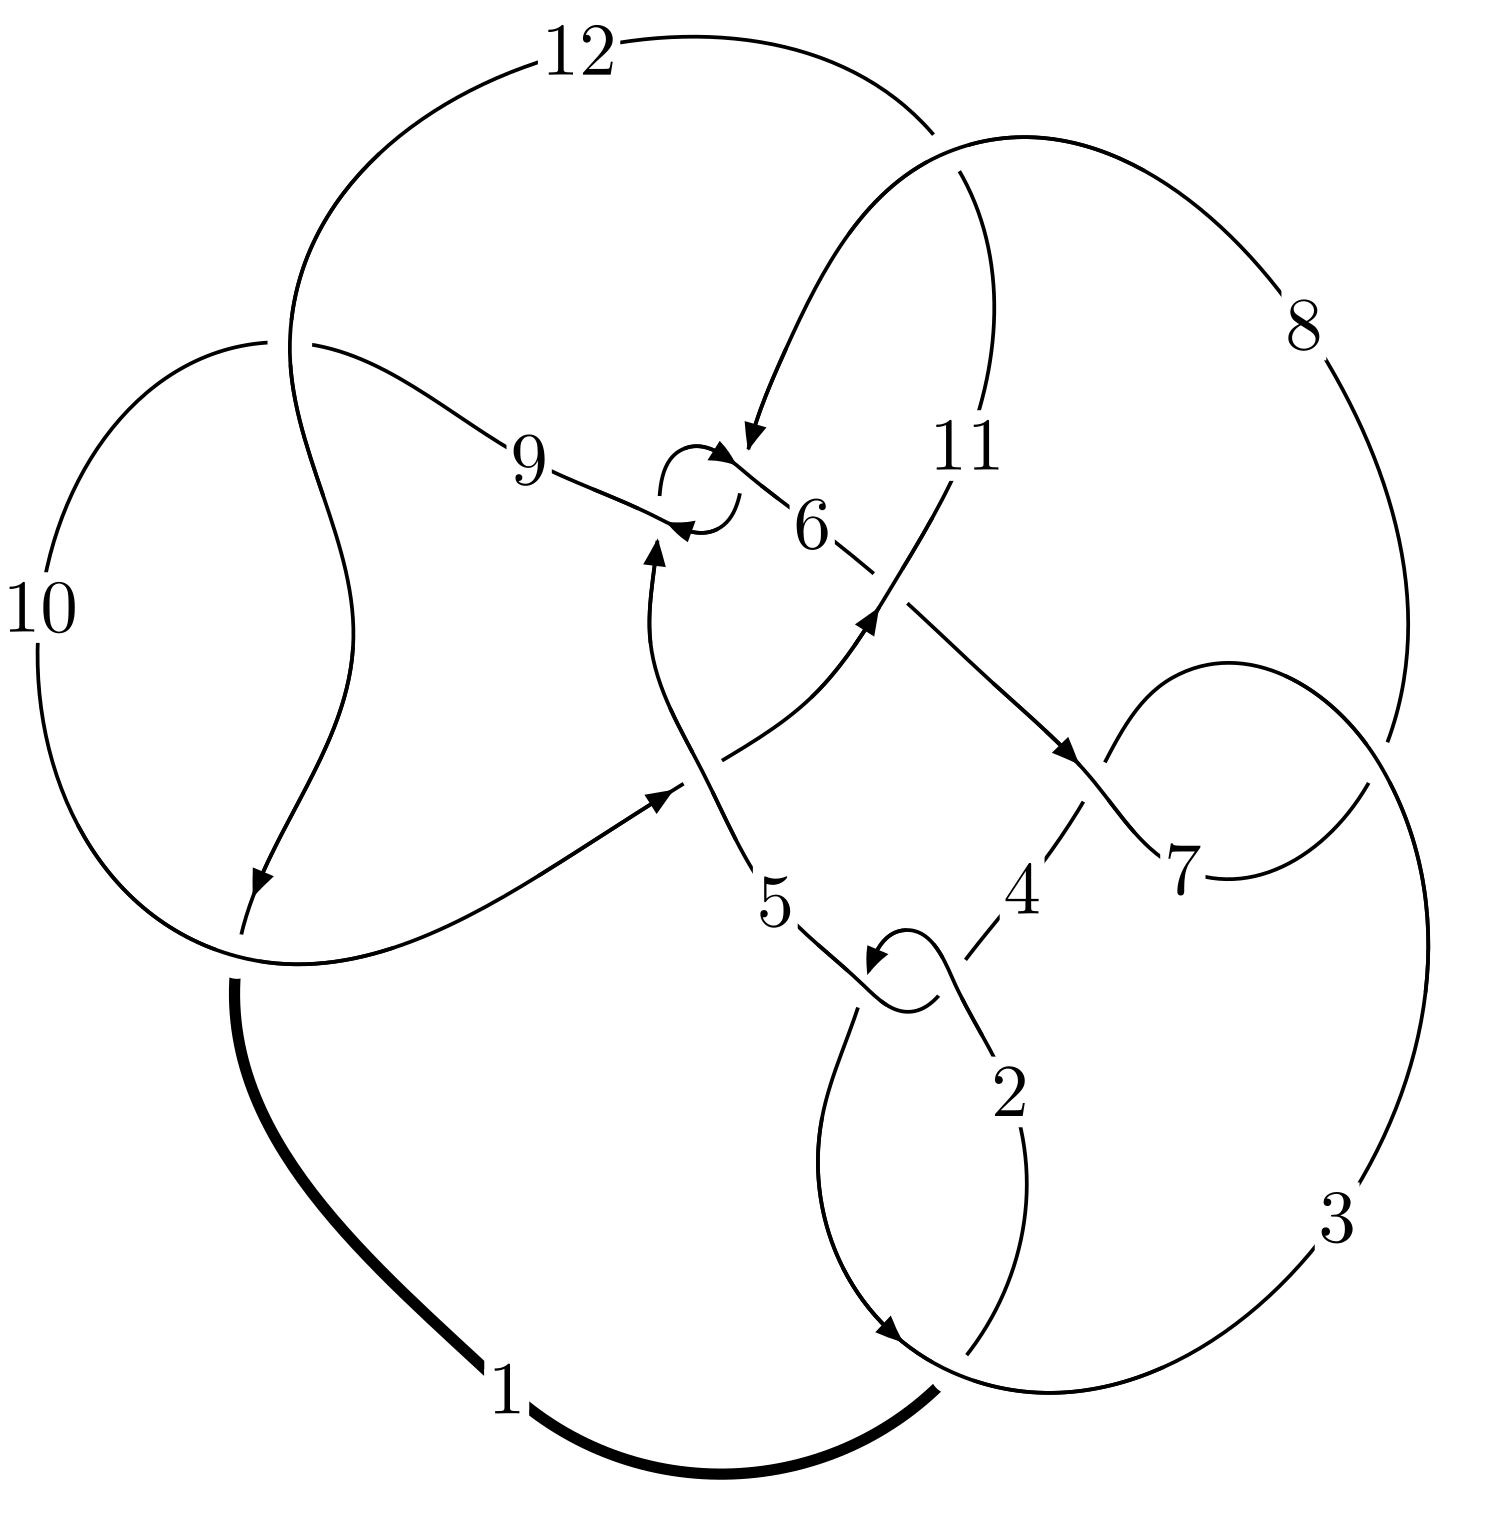
\includegraphics[width=112pt]{../../../GIT/diagram.site/Diagrams/png/2301_12n_0212.png}\\
\ \ \ A knot diagram\footnotemark}&
\allowdisplaybreaks
\textbf{Linearized knot diagam} \\
\cline{2-2}
 &
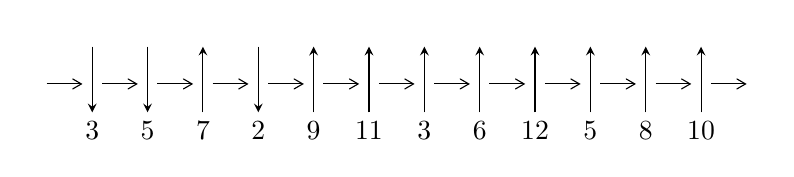
\begin{tikzpicture}[x=20pt, y=17pt]
	% nodes
	\node (C0) at (0, 0) {};
	\node (C1) at (1, 0) {};
	\node (C1U) at (1, +1) {};
	\node (C1D) at (1, -1) {3};

	\node (C2) at (2, 0) {};
	\node (C2U) at (2, +1) {};
	\node (C2D) at (2, -1) {5};

	\node (C3) at (3, 0) {};
	\node (C3U) at (3, +1) {};
	\node (C3D) at (3, -1) {7};

	\node (C4) at (4, 0) {};
	\node (C4U) at (4, +1) {};
	\node (C4D) at (4, -1) {2};

	\node (C5) at (5, 0) {};
	\node (C5U) at (5, +1) {};
	\node (C5D) at (5, -1) {9};

	\node (C6) at (6, 0) {};
	\node (C6U) at (6, +1) {};
	\node (C6D) at (6, -1) {11};

	\node (C7) at (7, 0) {};
	\node (C7U) at (7, +1) {};
	\node (C7D) at (7, -1) {3};

	\node (C8) at (8, 0) {};
	\node (C8U) at (8, +1) {};
	\node (C8D) at (8, -1) {6};

	\node (C9) at (9, 0) {};
	\node (C9U) at (9, +1) {};
	\node (C9D) at (9, -1) {12};

	\node (C10) at (10, 0) {};
	\node (C10U) at (10, +1) {};
	\node (C10D) at (10, -1) {5};

	\node (C11) at (11, 0) {};
	\node (C11U) at (11, +1) {};
	\node (C11D) at (11, -1) {8};

	\node (C12) at (12, 0) {};
	\node (C12U) at (12, +1) {};
	\node (C12D) at (12, -1) {10};
	\node (C13) at (13, 0) {};

	% arrows
	\draw[->,>={angle 60}]
	(C0) edge (C1) (C1) edge (C2) (C2) edge (C3) (C3) edge (C4) (C4) edge (C5) (C5) edge (C6) (C6) edge (C7) (C7) edge (C8) (C8) edge (C9) (C9) edge (C10) (C10) edge (C11) (C11) edge (C12) (C12) edge (C13) ;	\draw[->,>=stealth]
	(C1U) edge (C1D) (C2U) edge (C2D) (C3D) edge (C3U) (C4U) edge (C4D) (C5D) edge (C5U) (C6D) edge (C6U) (C7D) edge (C7U) (C8D) edge (C8U) (C9D) edge (C9U) (C10D) edge (C10U) (C11D) edge (C11U) (C12D) edge (C12U) ;
	\end{tikzpicture} \\
\hhline{~~} \\& 
\textbf{Solving Sequence} \\ \cline{2-2} 
 &
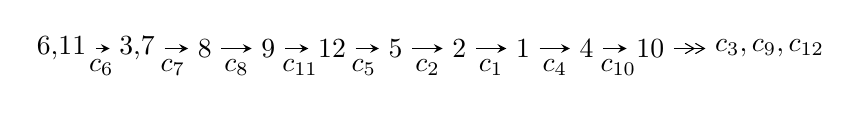
\begin{tikzpicture}[x=23pt, y=7pt]
	% node
	\node (A0) at (-1/8, 0) {6,11};
	\node (A1) at (17/16, 0) {3,7};
	\node (A2) at (17/8, 0) {8};
	\node (A3) at (25/8, 0) {9};
	\node (A4) at (33/8, 0) {12};
	\node (A5) at (41/8, 0) {5};
	\node (A6) at (49/8, 0) {2};
	\node (A7) at (57/8, 0) {1};
	\node (A8) at (65/8, 0) {4};
	\node (A9) at (73/8, 0) {10};
	\node (C1) at (1/2, -1) {$c_{6}$};
	\node (C2) at (13/8, -1) {$c_{7}$};
	\node (C3) at (21/8, -1) {$c_{8}$};
	\node (C4) at (29/8, -1) {$c_{11}$};
	\node (C5) at (37/8, -1) {$c_{5}$};
	\node (C6) at (45/8, -1) {$c_{2}$};
	\node (C7) at (53/8, -1) {$c_{1}$};
	\node (C8) at (61/8, -1) {$c_{4}$};
	\node (C9) at (69/8, -1) {$c_{10}$};
	\node (A10) at (11, 0) {$c_{3},c_{9},c_{12}$};

	% edge
	\draw[->,>=stealth]	
	(A0) edge (A1) (A1) edge (A2) (A2) edge (A3) (A3) edge (A4) (A4) edge (A5) (A5) edge (A6) (A6) edge (A7) (A7) edge (A8) (A8) edge (A9) ;
	\draw[->>,>={angle 60}]	
	(A9) edge (A10);
\end{tikzpicture} \\ 

\end{tabular} \\

\footnotetext{
The image of knot diagram is generated by the software ``\textbf{Draw programme}" developed by Andrew Bartholomew(\url{http://www.layer8.co.uk/maths/draw/index.htm\#Running-draw}), where we modified some parts for our purpose(\url{https://github.com/CATsTAILs/LinksPainter}).
}\phantom \\ \newline 
\centering \textbf{Ideals for irreducible components\footnotemark of $X_{\text{par}}$} 
 
\begin{align*}
I^u_{1}&=\langle 
-1.43322\times10^{268} u^{64}+4.87957\times10^{268} u^{63}+\cdots+4.09619\times10^{272} b+8.91816\times10^{272},\\
\phantom{I^u_{1}}&\phantom{= \langle  }2.78500\times10^{270} u^{64}-6.50544\times10^{270} u^{63}+\cdots+7.37313\times10^{273} a-4.93581\times10^{274},\\
\phantom{I^u_{1}}&\phantom{= \langle  }u^{65}-2 u^{64}+\cdots-19008 u+5184\rangle \\
I^u_{2}&=\langle 
u^6- u^4+u^2+b- u,\;u^7+u^6- u^5-3 u^4+u^3+3 u^2+a-3,\;u^8+u^7- u^6-2 u^5+u^4+2 u^3-2 u-1\rangle \\
\\
I^v_{1}&=\langle 
a,\;-18315 v^5+20514 v^4-76517 v^3+68962 v^2+11867 b+4895 v+9310,\\
\phantom{I^v_{1}}&\phantom{= \langle  }9 v^6-3 v^5+38 v^4-6 v^3+7 v^2-3 v+1\rangle \\
\end{align*}
\raggedright * 3 irreducible components of $\dim_{\mathbb{C}}=0$, with total 79 representations.\\
\footnotetext{All coefficients of polynomials are rational numbers. But the coefficients are sometimes approximated in decimal forms when there is not enough margin.}
\newpage
\renewcommand{\arraystretch}{1}
\centering \section*{I. $I^u_{1}= \langle -1.43\times10^{268} u^{64}+4.88\times10^{268} u^{63}+\cdots+4.10\times10^{272} b+8.92\times10^{272},\;2.79\times10^{270} u^{64}-6.51\times10^{270} u^{63}+\cdots+7.37\times10^{273} a-4.94\times10^{274},\;u^{65}-2 u^{64}+\cdots-19008 u+5184 \rangle$}
\flushleft \textbf{(i) Arc colorings}\\
\begin{tabular}{m{7pt} m{180pt} m{7pt} m{180pt} }
\flushright $a_{6}=$&$\begin{pmatrix}1\\0\end{pmatrix}$ \\
\flushright $a_{11}=$&$\begin{pmatrix}0\\u\end{pmatrix}$ \\
\flushright $a_{3}=$&$\begin{pmatrix}-0.000377723 u^{64}+0.000882317 u^{63}+\cdots-24.2190 u+6.69432\\0.0000349893 u^{64}-0.000119125 u^{63}+\cdots+6.31596 u-2.17719\end{pmatrix}$ \\
\flushright $a_{7}=$&$\begin{pmatrix}1\\- u^2\end{pmatrix}$ \\
\flushright $a_{8}=$&$\begin{pmatrix}-0.000281496 u^{64}+0.000444213 u^{63}+\cdots-2.66344 u-1.87984\\0.0000716784 u^{64}-0.0000602668 u^{63}+\cdots-2.06803 u+1.30681\end{pmatrix}$ \\
\flushright $a_{9}=$&$\begin{pmatrix}-0.000209817 u^{64}+0.000383947 u^{63}+\cdots-4.73147 u-0.573035\\0.0000716784 u^{64}-0.0000602668 u^{63}+\cdots-2.06803 u+1.30681\end{pmatrix}$ \\
\flushright $a_{12}=$&$\begin{pmatrix}0.000110706 u^{64}-0.000268775 u^{63}+\cdots+6.05995 u-1.93909\\0.000214065 u^{64}-0.000335465 u^{63}+\cdots+2.94068 u+0.325061\end{pmatrix}$ \\
\flushright $a_{5}=$&$\begin{pmatrix}0.0000382070 u^{64}+0.0000348721 u^{63}+\cdots-4.30269 u+2.47351\\0.000100912 u^{64}-0.000304602 u^{63}+\cdots+8.12093 u-1.65906\end{pmatrix}$ \\
\flushright $a_{2}=$&$\begin{pmatrix}-0.000284710 u^{64}+0.000546492 u^{63}+\cdots-12.1877 u+2.72060\\0.000172387 u^{64}-0.000396564 u^{63}+\cdots+8.99806 u-2.35482\end{pmatrix}$ \\
\flushright $a_{1}=$&$\begin{pmatrix}0.000100309 u^{64}-0.000149136 u^{63}+\cdots+0.894466 u-0.119551\\-0.000143803 u^{64}+0.000150522 u^{63}+\cdots+1.65869 u-1.49182\end{pmatrix}$ \\
\flushright $a_{4}=$&$\begin{pmatrix}-0.000313975 u^{64}+0.000618260 u^{63}+\cdots-13.5334 u+3.85944\\0.0000715938 u^{64}-0.000222008 u^{63}+\cdots+9.24221 u-2.88513\end{pmatrix}$ \\
\flushright $a_{10}=$&$\begin{pmatrix}0.000148358 u^{64}-0.000310823 u^{63}+\cdots+4.46935 u-2.06733\\0.000108769 u^{64}-0.000131377 u^{63}+\cdots+0.525836 u+0.505205\end{pmatrix}$\\&\end{tabular}
\flushleft \textbf{(ii) Obstruction class $= -1$}\\~\\
\flushleft \textbf{(iii) Cusp Shapes $= -0.00132072 u^{64}+0.00246498 u^{63}+\cdots-45.0317 u+16.1770$}\\~\\
\newpage\renewcommand{\arraystretch}{1}
\flushleft \textbf{(iv) u-Polynomials at the component}\newline \\
\begin{tabular}{m{50pt}|m{274pt}}
Crossings & \hspace{64pt}u-Polynomials at each crossing \\
\hline $$\begin{aligned}c_{1}\end{aligned}$$&$\begin{aligned}
&u^{65}+68 u^{64}+\cdots+59 u+1
\end{aligned}$\\
\hline $$\begin{aligned}c_{2},c_{4}\end{aligned}$$&$\begin{aligned}
&u^{65}-10 u^{64}+\cdots-11 u+1
\end{aligned}$\\
\hline $$\begin{aligned}c_{3},c_{7}\end{aligned}$$&$\begin{aligned}
&u^{65}-2 u^{64}+\cdots+640 u-256
\end{aligned}$\\
\hline $$\begin{aligned}c_{5},c_{8}\end{aligned}$$&$\begin{aligned}
&u^{65}+3 u^{64}+\cdots+3 u+1
\end{aligned}$\\
\hline $$\begin{aligned}c_{6}\end{aligned}$$&$\begin{aligned}
&u^{65}+2 u^{64}+\cdots-19008 u-5184
\end{aligned}$\\
\hline $$\begin{aligned}c_{9},c_{12}\end{aligned}$$&$\begin{aligned}
&u^{65}+8 u^{64}+\cdots+1080 u+81
\end{aligned}$\\
\hline $$\begin{aligned}c_{10}\end{aligned}$$&$\begin{aligned}
&9(9 u^{65}+18 u^{64}+\cdots-294572 u-29917)
\end{aligned}$\\
\hline $$\begin{aligned}c_{11}\end{aligned}$$&$\begin{aligned}
&9(9 u^{65}+42 u^{64}+\cdots+608293 u+315227)
\end{aligned}$\\
\hline
\end{tabular}\\~\\
\newpage\renewcommand{\arraystretch}{1}
\flushleft \textbf{(v) Riley Polynomials at the component}\newline \\
\begin{tabular}{m{50pt}|m{274pt}}
Crossings & \hspace{64pt}Riley Polynomials at each crossing \\
\hline $$\begin{aligned}c_{1}\end{aligned}$$&$\begin{aligned}
&y^{65}-132 y^{64}+\cdots+7503 y-1
\end{aligned}$\\
\hline $$\begin{aligned}c_{2},c_{4}\end{aligned}$$&$\begin{aligned}
&y^{65}-68 y^{64}+\cdots+59 y-1
\end{aligned}$\\
\hline $$\begin{aligned}c_{3},c_{7}\end{aligned}$$&$\begin{aligned}
&y^{65}+48 y^{64}+\cdots+901120 y-65536
\end{aligned}$\\
\hline $$\begin{aligned}c_{5},c_{8}\end{aligned}$$&$\begin{aligned}
&y^{65}+37 y^{64}+\cdots+11 y-1
\end{aligned}$\\
\hline $$\begin{aligned}c_{6}\end{aligned}$$&$\begin{aligned}
&y^{65}+36 y^{64}+\cdots-462827520 y-26873856
\end{aligned}$\\
\hline $$\begin{aligned}c_{9},c_{12}\end{aligned}$$&$\begin{aligned}
&y^{65}-30 y^{64}+\cdots+422172 y-6561
\end{aligned}$\\
\hline $$\begin{aligned}c_{10}\end{aligned}$$&$\begin{aligned}
&81(81 y^{65}+5796 y^{64}+\cdots+1.08032\times10^{10} y-8.95027\times10^{8})
\end{aligned}$\\
\hline $$\begin{aligned}c_{11}\end{aligned}$$&$\begin{aligned}
&81(81 y^{65}-558 y^{64}+\cdots-1.06335\times10^{12} y-9.93681\times10^{10})
\end{aligned}$\\
\hline
\end{tabular}\\~\\
\newpage\flushleft \textbf{(vi) Complex Volumes and Cusp Shapes}
$$\begin{array}{c|c|c}  
\text{Solutions to }I^u_{1}& \I (\text{vol} + \sqrt{-1}CS) & \text{Cusp shape}\\
 \hline 
\begin{aligned}
u &= -0.987989 + 0.000953 I \\
a &= -2.12082 + 1.54640 I \\
b &= \phantom{-}1.33246 - 1.66976 I\end{aligned}
 & -2.66486 - 2.32248 I & \phantom{-}5.14580 + 2.29349 I \\ \hline\begin{aligned}
u &= -0.987989 - 0.000953 I \\
a &= -2.12082 - 1.54640 I \\
b &= \phantom{-}1.33246 + 1.66976 I\end{aligned}
 & -2.66486 + 2.32248 I & \phantom{-}5.14580 - 2.29349 I \\ \hline\begin{aligned}
u &= -0.748540 + 0.696645 I \\
a &= \phantom{-}0.226780 + 1.145830 I \\
b &= -0.874173 - 0.089609 I\end{aligned}
 & \phantom{-}1.04936 + 1.32007 I & \phantom{-}10.95788 - 0.41796 I \\ \hline\begin{aligned}
u &= -0.748540 - 0.696645 I \\
a &= \phantom{-}0.226780 - 1.145830 I \\
b &= -0.874173 + 0.089609 I\end{aligned}
 & \phantom{-}1.04936 - 1.32007 I & \phantom{-}10.95788 + 0.41796 I \\ \hline\begin{aligned}
u &= \phantom{-}0.055143 + 1.022190 I \\
a &= \phantom{-}0.05532 - 1.41633 I \\
b &= -0.271016 - 0.120884 I\end{aligned}
 & -2.21134 + 0.65096 I & \phantom{-}2.94304 - 0.27515 I \\ \hline\begin{aligned}
u &= \phantom{-}0.055143 - 1.022190 I \\
a &= \phantom{-}0.05532 + 1.41633 I \\
b &= -0.271016 + 0.120884 I\end{aligned}
 & -2.21134 - 0.65096 I & \phantom{-}2.94304 + 0.27515 I \\ \hline\begin{aligned}
u &= \phantom{-}0.963379\phantom{ +0.000000I} \\
a &= -0.0469319\phantom{ +0.000000I} \\
b &= \phantom{-}0.578355\phantom{ +0.000000I}\end{aligned}
 & \phantom{-}5.22479\phantom{ +0.000000I} & \phantom{-}24.0830\phantom{ +0.000000I} \\ \hline\begin{aligned}
u &= -0.286459 + 1.010510 I \\
a &= \phantom{-}0.78431 + 1.39006 I \\
b &= -0.316087 + 1.221670 I\end{aligned}
 & \phantom{-}1.45815 + 1.19485 I & \phantom{-}9.19775 - 4.74594 I \\ \hline\begin{aligned}
u &= -0.286459 - 1.010510 I \\
a &= \phantom{-}0.78431 - 1.39006 I \\
b &= -0.316087 - 1.221670 I\end{aligned}
 & \phantom{-}1.45815 - 1.19485 I & \phantom{-}9.19775 + 4.74594 I \\ \hline\begin{aligned}
u &= \phantom{-}0.726229 + 0.814196 I \\
a &= -0.121481 - 0.226198 I \\
b &= -0.807017 + 0.074160 I\end{aligned}
 & -2.55567 + 2.51492 I & \phantom{-}6.00000 - 3.00902 I\\
 \hline 
 \end{array}$$\newpage$$\begin{array}{c|c|c}  
\text{Solutions to }I^u_{1}& \I (\text{vol} + \sqrt{-1}CS) & \text{Cusp shape}\\
 \hline 
\begin{aligned}
u &= \phantom{-}0.726229 - 0.814196 I \\
a &= -0.121481 + 0.226198 I \\
b &= -0.807017 - 0.074160 I\end{aligned}
 & -2.55567 - 2.51492 I & \phantom{-}6.00000 + 3.00902 I \\ \hline\begin{aligned}
u &= -0.891332 + 0.686560 I \\
a &= \phantom{-}0.0513899 - 0.0389433 I \\
b &= -0.565696 + 0.133789 I\end{aligned}
 & \phantom{-}1.17561 - 6.59366 I & \phantom{-}15.1731 + 8.7497 I \\ \hline\begin{aligned}
u &= -0.891332 - 0.686560 I \\
a &= \phantom{-}0.0513899 + 0.0389433 I \\
b &= -0.565696 - 0.133789 I\end{aligned}
 & \phantom{-}1.17561 + 6.59366 I & \phantom{-}15.1731 - 8.7497 I \\ \hline\begin{aligned}
u &= \phantom{-}0.218273 + 1.185850 I \\
a &= -0.011907 - 0.174978 I \\
b &= -1.58075 + 0.11150 I\end{aligned}
 & -3.79735 + 2.57206 I & \phantom{-0.000000 } 0 \\ \hline\begin{aligned}
u &= \phantom{-}0.218273 - 1.185850 I \\
a &= -0.011907 + 0.174978 I \\
b &= -1.58075 - 0.11150 I\end{aligned}
 & -3.79735 - 2.57206 I & \phantom{-0.000000 } 0 \\ \hline\begin{aligned}
u &= -0.627540 + 0.484254 I \\
a &= \phantom{-}1.321520 + 0.352976 I \\
b &= -0.573718 + 0.068027 I\end{aligned}
 & \phantom{-}1.19155 + 0.95389 I & \phantom{-}10.21513 - 0.37317 I \\ \hline\begin{aligned}
u &= -0.627540 - 0.484254 I \\
a &= \phantom{-}1.321520 - 0.352976 I \\
b &= -0.573718 - 0.068027 I\end{aligned}
 & \phantom{-}1.19155 - 0.95389 I & \phantom{-}10.21513 + 0.37317 I \\ \hline\begin{aligned}
u &= -0.485202 + 1.151820 I \\
a &= \phantom{-}0.294894 + 1.249500 I \\
b &= -0.567218 + 0.263601 I\end{aligned}
 & -0.92912 - 5.51849 I & \phantom{-0.000000 } 0 \\ \hline\begin{aligned}
u &= -0.485202 - 1.151820 I \\
a &= \phantom{-}0.294894 - 1.249500 I \\
b &= -0.567218 - 0.263601 I\end{aligned}
 & -0.92912 + 5.51849 I & \phantom{-0.000000 } 0 \\ \hline\begin{aligned}
u &= -0.001950 + 1.261610 I \\
a &= -0.529291 + 1.160890 I \\
b &= -1.249780 + 0.587678 I\end{aligned}
 & -5.91253 + 0.89151 I & \phantom{-0.000000 } 0\\
 \hline 
 \end{array}$$\newpage$$\begin{array}{c|c|c}  
\text{Solutions to }I^u_{1}& \I (\text{vol} + \sqrt{-1}CS) & \text{Cusp shape}\\
 \hline 
\begin{aligned}
u &= -0.001950 - 1.261610 I \\
a &= -0.529291 - 1.160890 I \\
b &= -1.249780 - 0.587678 I\end{aligned}
 & -5.91253 - 0.89151 I & \phantom{-0.000000 } 0 \\ \hline\begin{aligned}
u &= -0.181767 + 1.284800 I \\
a &= \phantom{-}0.394438 + 1.295480 I \\
b &= \phantom{-}0.520041 + 0.490473 I\end{aligned}
 & -13.75280 + 0.18156 I & \phantom{-0.000000 } 0 \\ \hline\begin{aligned}
u &= -0.181767 - 1.284800 I \\
a &= \phantom{-}0.394438 - 1.295480 I \\
b &= \phantom{-}0.520041 - 0.490473 I\end{aligned}
 & -13.75280 - 0.18156 I & \phantom{-0.000000 } 0 \\ \hline\begin{aligned}
u &= \phantom{-}0.666243 + 0.215627 I \\
a &= \phantom{-}0.63298 + 3.14043 I \\
b &= \phantom{-}0.528259 + 0.129647 I\end{aligned}
 & -9.22847 - 0.59840 I & \phantom{-}0.51834 - 6.09970 I \\ \hline\begin{aligned}
u &= \phantom{-}0.666243 - 0.215627 I \\
a &= \phantom{-}0.63298 - 3.14043 I \\
b &= \phantom{-}0.528259 - 0.129647 I\end{aligned}
 & -9.22847 + 0.59840 I & \phantom{-}0.51834 + 6.09970 I \\ \hline\begin{aligned}
u &= \phantom{-}0.667926 + 0.125084 I \\
a &= \phantom{-}3.07822 - 0.34270 I \\
b &= -1.44314 + 0.42007 I\end{aligned}
 & -1.45078 - 0.59119 I & \phantom{-}2.85675 - 3.51070 I \\ \hline\begin{aligned}
u &= \phantom{-}0.667926 - 0.125084 I \\
a &= \phantom{-}3.07822 + 0.34270 I \\
b &= -1.44314 - 0.42007 I\end{aligned}
 & -1.45078 + 0.59119 I & \phantom{-}2.85675 + 3.51070 I \\ \hline\begin{aligned}
u &= \phantom{-}0.375714 + 1.275330 I \\
a &= -0.01142 - 1.46097 I \\
b &= -1.39649 - 0.60732 I\end{aligned}
 & -5.14289 + 4.65238 I & \phantom{-0.000000 } 0 \\ \hline\begin{aligned}
u &= \phantom{-}0.375714 - 1.275330 I \\
a &= -0.01142 + 1.46097 I \\
b &= -1.39649 + 0.60732 I\end{aligned}
 & -5.14289 - 4.65238 I & \phantom{-0.000000 } 0 \\ \hline\begin{aligned}
u &= \phantom{-}1.370430 + 0.169263 I \\
a &= -0.311596 + 0.742406 I \\
b &= \phantom{-}1.14616 - 2.08345 I\end{aligned}
 & -0.61197 - 3.88642 I & \phantom{-0.000000 } 0\\
 \hline 
 \end{array}$$\newpage$$\begin{array}{c|c|c}  
\text{Solutions to }I^u_{1}& \I (\text{vol} + \sqrt{-1}CS) & \text{Cusp shape}\\
 \hline 
\begin{aligned}
u &= \phantom{-}1.370430 - 0.169263 I \\
a &= -0.311596 - 0.742406 I \\
b &= \phantom{-}1.14616 + 2.08345 I\end{aligned}
 & -0.61197 + 3.88642 I & \phantom{-0.000000 } 0 \\ \hline\begin{aligned}
u &= \phantom{-}0.224303 + 0.571448 I \\
a &= \phantom{-}1.08323 - 6.98590 I \\
b &= -1.15343 - 1.78571 I\end{aligned}
 & -0.766193 - 0.710691 I & -8.2875 - 12.4812 I \\ \hline\begin{aligned}
u &= \phantom{-}0.224303 - 0.571448 I \\
a &= \phantom{-}1.08323 + 6.98590 I \\
b &= -1.15343 + 1.78571 I\end{aligned}
 & -0.766193 + 0.710691 I & -8.2875 + 12.4812 I \\ \hline\begin{aligned}
u &= -0.271460 + 0.550386 I \\
a &= \phantom{-}0.171011 - 0.156416 I \\
b &= -1.073610 + 0.399773 I\end{aligned}
 & \phantom{-}1.52187 - 6.09633 I & \phantom{-}2.3393 + 14.1949 I \\ \hline\begin{aligned}
u &= -0.271460 - 0.550386 I \\
a &= \phantom{-}0.171011 + 0.156416 I \\
b &= -1.073610 - 0.399773 I\end{aligned}
 & \phantom{-}1.52187 + 6.09633 I & \phantom{-}2.3393 - 14.1949 I \\ \hline\begin{aligned}
u &= \phantom{-}0.553293 + 1.271240 I \\
a &= \phantom{-}0.553265 - 0.871213 I \\
b &= \phantom{-}0.249245 - 0.493678 I\end{aligned}
 & -12.27680 + 5.48243 I & \phantom{-0.000000 } 0 \\ \hline\begin{aligned}
u &= \phantom{-}0.553293 - 1.271240 I \\
a &= \phantom{-}0.553265 + 0.871213 I \\
b &= \phantom{-}0.249245 + 0.493678 I\end{aligned}
 & -12.27680 - 5.48243 I & \phantom{-0.000000 } 0 \\ \hline\begin{aligned}
u &= \phantom{-}0.060757 + 0.566257 I \\
a &= -0.169552 + 0.223408 I \\
b &= \phantom{-}1.169990 - 0.272700 I\end{aligned}
 & \phantom{-}3.05269 - 0.72062 I & -0.37252 - 2.34749 I \\ \hline\begin{aligned}
u &= \phantom{-}0.060757 - 0.566257 I \\
a &= -0.169552 - 0.223408 I \\
b &= \phantom{-}1.169990 + 0.272700 I\end{aligned}
 & \phantom{-}3.05269 + 0.72062 I & -0.37252 + 2.34749 I \\ \hline\begin{aligned}
u &= -0.541890\phantom{ +0.000000I} \\
a &= \phantom{-}0.432973\phantom{ +0.000000I} \\
b &= \phantom{-}0.203067\phantom{ +0.000000I}\end{aligned}
 & \phantom{-}0.709590\phantom{ +0.000000I} & \phantom{-}14.3470\phantom{ +0.000000I}\\
 \hline 
 \end{array}$$\newpage$$\begin{array}{c|c|c}  
\text{Solutions to }I^u_{1}& \I (\text{vol} + \sqrt{-1}CS) & \text{Cusp shape}\\
 \hline 
\begin{aligned}
u &= \phantom{-}0.22284 + 1.47296 I \\
a &= \phantom{-}0.233664 + 0.102031 I \\
b &= \phantom{-}1.89702 + 0.23201 I\end{aligned}
 & -8.45370 + 1.77642 I & \phantom{-0.000000 } 0 \\ \hline\begin{aligned}
u &= \phantom{-}0.22284 - 1.47296 I \\
a &= \phantom{-}0.233664 - 0.102031 I \\
b &= \phantom{-}1.89702 - 0.23201 I\end{aligned}
 & -8.45370 - 1.77642 I & \phantom{-0.000000 } 0 \\ \hline\begin{aligned}
u &= -0.53597 + 1.39821 I \\
a &= -0.146182 - 0.038643 I \\
b &= \phantom{-}1.399900 - 0.050013 I\end{aligned}
 & -7.04530 - 8.03742 I & \phantom{-0.000000 } 0 \\ \hline\begin{aligned}
u &= -0.53597 - 1.39821 I \\
a &= -0.146182 + 0.038643 I \\
b &= \phantom{-}1.399900 + 0.050013 I\end{aligned}
 & -7.04530 + 8.03742 I & \phantom{-0.000000 } 0 \\ \hline\begin{aligned}
u &= \phantom{-}0.497138\phantom{ +0.000000I} \\
a &= \phantom{-}6.35919\phantom{ +0.000000I} \\
b &= -1.12723\phantom{ +0.000000I}\end{aligned}
 & -0.408756\phantom{ +0.000000I} & \phantom{-}31.3810\phantom{ +0.000000I} \\ \hline\begin{aligned}
u &= \phantom{-}0.72094 + 1.40121 I \\
a &= -0.313940 + 1.369360 I \\
b &= \phantom{-}1.89330 + 1.11991 I\end{aligned}
 & -4.34514 + 11.16830 I & \phantom{-0.000000 } 0 \\ \hline\begin{aligned}
u &= \phantom{-}0.72094 - 1.40121 I \\
a &= -0.313940 - 1.369360 I \\
b &= \phantom{-}1.89330 - 1.11991 I\end{aligned}
 & -4.34514 - 11.16830 I & \phantom{-0.000000 } 0 \\ \hline\begin{aligned}
u &= \phantom{-}0.097484 + 0.387248 I \\
a &= \phantom{-}0.01203 - 2.23100 I \\
b &= -0.493159 + 0.407995 I\end{aligned}
 & -1.70444 + 0.86317 I & -1.80335 - 2.14625 I \\ \hline\begin{aligned}
u &= \phantom{-}0.097484 - 0.387248 I \\
a &= \phantom{-}0.01203 + 2.23100 I \\
b &= -0.493159 - 0.407995 I\end{aligned}
 & -1.70444 - 0.86317 I & -1.80335 + 2.14625 I \\ \hline\begin{aligned}
u &= -0.88341 + 1.34912 I \\
a &= -0.447992 - 1.029800 I \\
b &= \phantom{-}1.177480 - 0.641815 I\end{aligned}
 & -7.46828 - 10.68780 I & \phantom{-0.000000 } 0\\
 \hline 
 \end{array}$$\newpage$$\begin{array}{c|c|c}  
\text{Solutions to }I^u_{1}& \I (\text{vol} + \sqrt{-1}CS) & \text{Cusp shape}\\
 \hline 
\begin{aligned}
u &= -0.88341 - 1.34912 I \\
a &= -0.447992 + 1.029800 I \\
b &= \phantom{-}1.177480 + 0.641815 I\end{aligned}
 & -7.46828 + 10.68780 I & \phantom{-0.000000 } 0 \\ \hline\begin{aligned}
u &= -0.51591 + 1.53296 I \\
a &= \phantom{-}0.030967 - 1.340990 I \\
b &= \phantom{-}2.10343 - 1.45671 I\end{aligned}
 & -6.56044 - 4.64446 I & \phantom{-0.000000 } 0 \\ \hline\begin{aligned}
u &= -0.51591 - 1.53296 I \\
a &= \phantom{-}0.030967 + 1.340990 I \\
b &= \phantom{-}2.10343 + 1.45671 I\end{aligned}
 & -6.56044 + 4.64446 I & \phantom{-0.000000 } 0 \\ \hline\begin{aligned}
u &= \phantom{-}0.82368 + 1.39986 I \\
a &= -0.450753 + 0.978865 I \\
b &= \phantom{-}1.237730 + 0.645893 I\end{aligned}
 & -10.53090 + 4.21781 I & \phantom{-0.000000 } 0 \\ \hline\begin{aligned}
u &= \phantom{-}0.82368 - 1.39986 I \\
a &= -0.450753 - 0.978865 I \\
b &= \phantom{-}1.237730 - 0.645893 I\end{aligned}
 & -10.53090 - 4.21781 I & \phantom{-0.000000 } 0 \\ \hline\begin{aligned}
u &= -1.52984 + 0.86914 I \\
a &= -0.354905 - 0.297066 I \\
b &= \phantom{-}1.52741 + 0.94608 I\end{aligned}
 & -5.31966 + 2.30754 I & \phantom{-0.000000 } 0 \\ \hline\begin{aligned}
u &= -1.52984 - 0.86914 I \\
a &= -0.354905 + 0.297066 I \\
b &= \phantom{-}1.52741 - 0.94608 I\end{aligned}
 & -5.31966 - 2.30754 I & \phantom{-0.000000 } 0 \\ \hline\begin{aligned}
u &= \phantom{-}0.99000 + 1.57649 I \\
a &= \phantom{-}0.478911 - 1.130600 I \\
b &= -2.01241 - 1.65324 I\end{aligned}
 & -11.1904 + 16.3453 I & \phantom{-0.000000 } 0 \\ \hline\begin{aligned}
u &= \phantom{-}0.99000 - 1.57649 I \\
a &= \phantom{-}0.478911 + 1.130600 I \\
b &= -2.01241 + 1.65324 I\end{aligned}
 & -11.1904 - 16.3453 I & \phantom{-0.000000 } 0 \\ \hline\begin{aligned}
u &= -0.65125 + 2.02422 I \\
a &= -0.213696 - 0.852249 I \\
b &= \phantom{-}1.51737 - 2.34323 I\end{aligned}
 & -4.34300 + 1.86014 I & \phantom{-0.000000 } 0\\
 \hline 
 \end{array}$$\newpage$$\begin{array}{c|c|c}  
\text{Solutions to }I^u_{1}& \I (\text{vol} + \sqrt{-1}CS) & \text{Cusp shape}\\
 \hline 
\begin{aligned}
u &= -0.65125 - 2.02422 I \\
a &= -0.213696 + 0.852249 I \\
b &= \phantom{-}1.51737 + 2.34323 I\end{aligned}
 & -4.34300 - 1.86014 I & \phantom{-0.000000 } 0 \\ \hline\begin{aligned}
u &= -0.90018 + 2.02783 I \\
a &= \phantom{-}0.247259 + 0.974849 I \\
b &= -2.21700 + 2.52211 I\end{aligned}
 & -14.1808 - 8.5511 I & \phantom{-0.000000 } 0 \\ \hline\begin{aligned}
u &= -0.90018 - 2.02783 I \\
a &= \phantom{-}0.247259 - 0.974849 I \\
b &= -2.21700 - 2.52211 I\end{aligned}
 & -14.1808 + 8.5511 I & \phantom{-0.000000 } 0 \\ \hline\begin{aligned}
u &= \phantom{-}2.26622 + 0.12631 I \\
a &= -0.013705 - 0.386355 I \\
b &= -0.43221 + 3.40125 I\end{aligned}
 & -7.12119 - 6.12750 I & \phantom{-0.000000 } 0 \\ \hline\begin{aligned}
u &= \phantom{-}2.26622 - 0.12631 I \\
a &= -0.013705 + 0.386355 I \\
b &= -0.43221 - 3.40125 I\end{aligned}
 & -7.12119 + 6.12750 I & \phantom{-0.000000 } 0\\
 \hline 
 \end{array}$$\newpage\newpage\renewcommand{\arraystretch}{1}
\centering \section*{II. $I^u_{2}= \langle u^6- u^4+u^2+b- u,\;u^7+u^6- u^5-3 u^4+u^3+3 u^2+a-3,\;u^8+u^7- u^6-2 u^5+u^4+2 u^3-2 u-1 \rangle$}
\flushleft \textbf{(i) Arc colorings}\\
\begin{tabular}{m{7pt} m{180pt} m{7pt} m{180pt} }
\flushright $a_{6}=$&$\begin{pmatrix}1\\0\end{pmatrix}$ \\
\flushright $a_{11}=$&$\begin{pmatrix}0\\u\end{pmatrix}$ \\
\flushright $a_{3}=$&$\begin{pmatrix}- u^7- u^6+u^5+3 u^4- u^3-3 u^2+3\\- u^6+u^4- u^2+u\end{pmatrix}$ \\
\flushright $a_{7}=$&$\begin{pmatrix}1\\- u^2\end{pmatrix}$ \\
\flushright $a_{8}=$&$\begin{pmatrix}1\\- u^2\end{pmatrix}$ \\
\flushright $a_{9}=$&$\begin{pmatrix}- u^2+1\\- u^2\end{pmatrix}$ \\
\flushright $a_{12}=$&$\begin{pmatrix}u\\- u^3+u\end{pmatrix}$ \\
\flushright $a_{5}=$&$\begin{pmatrix}u^4- u^2+1\\u^4\end{pmatrix}$ \\
\flushright $a_{2}=$&$\begin{pmatrix}- u^7- u^6+u^5+2 u^4- u^3-2 u^2+2\\- u^6- u^2+u\end{pmatrix}$ \\
\flushright $a_{1}=$&$\begin{pmatrix}- u^4+u^2-1\\- u^4\end{pmatrix}$ \\
\flushright $a_{4}=$&$\begin{pmatrix}- u^7- u^6+u^5+3 u^4- u^3-3 u^2+3\\- u^6+u^4- u^2+u\end{pmatrix}$ \\
\flushright $a_{10}=$&$\begin{pmatrix}- u^6+u^4-2 u^2+1\\- u^7- u^6+2 u^5+u^4-2 u^3-2 u^2+2 u+1\end{pmatrix}$\\&\end{tabular}
\flushleft \textbf{(ii) Obstruction class $= 1$}\\~\\
\flushleft \textbf{(iii) Cusp Shapes $= u^7+4 u^6-2 u^5-5 u^4+3 u^3+5 u^2-5 u-2$}\\~\\
\newpage\renewcommand{\arraystretch}{1}
\flushleft \textbf{(iv) u-Polynomials at the component}\newline \\
\begin{tabular}{m{50pt}|m{274pt}}
Crossings & \hspace{64pt}u-Polynomials at each crossing \\
\hline $$\begin{aligned}c_{1},c_{2}\end{aligned}$$&$\begin{aligned}
&(u-1)^8
\end{aligned}$\\
\hline $$\begin{aligned}c_{3},c_{7}\end{aligned}$$&$\begin{aligned}
&u^8
\end{aligned}$\\
\hline $$\begin{aligned}c_{4}\end{aligned}$$&$\begin{aligned}
&(u+1)^8
\end{aligned}$\\
\hline $$\begin{aligned}c_{5}\end{aligned}$$&$\begin{aligned}
&u^8+3 u^7+7 u^6+10 u^5+11 u^4+10 u^3+6 u^2+4 u+1
\end{aligned}$\\
\hline $$\begin{aligned}c_{6}\end{aligned}$$&$\begin{aligned}
&u^8+u^7- u^6-2 u^5+u^4+2 u^3-2 u-1
\end{aligned}$\\
\hline $$\begin{aligned}c_{8}\end{aligned}$$&$\begin{aligned}
&u^8-3 u^7+7 u^6-10 u^5+11 u^4-10 u^3+6 u^2-4 u+1
\end{aligned}$\\
\hline $$\begin{aligned}c_{9}\end{aligned}$$&$\begin{aligned}
&u^8- u^7-3 u^6+2 u^5+3 u^4-2 u-1
\end{aligned}$\\
\hline $$\begin{aligned}c_{10},c_{12}\end{aligned}$$&$\begin{aligned}
&u^8+u^7-3 u^6-2 u^5+3 u^4+2 u-1
\end{aligned}$\\
\hline $$\begin{aligned}c_{11}\end{aligned}$$&$\begin{aligned}
&u^8- u^7- u^6+2 u^5+u^4-2 u^3+2 u-1
\end{aligned}$\\
\hline
\end{tabular}\\~\\
\newpage\renewcommand{\arraystretch}{1}
\flushleft \textbf{(v) Riley Polynomials at the component}\newline \\
\begin{tabular}{m{50pt}|m{274pt}}
Crossings & \hspace{64pt}Riley Polynomials at each crossing \\
\hline $$\begin{aligned}c_{1},c_{2},c_{4}\end{aligned}$$&$\begin{aligned}
&(y-1)^8
\end{aligned}$\\
\hline $$\begin{aligned}c_{3},c_{7}\end{aligned}$$&$\begin{aligned}
&y^8
\end{aligned}$\\
\hline $$\begin{aligned}c_{5},c_{8}\end{aligned}$$&$\begin{aligned}
&y^8+5 y^7+11 y^6+6 y^5-17 y^4-34 y^3-22 y^2-4 y+1
\end{aligned}$\\
\hline $$\begin{aligned}c_{6},c_{11}\end{aligned}$$&$\begin{aligned}
&y^8-3 y^7+7 y^6-10 y^5+11 y^4-10 y^3+6 y^2-4 y+1
\end{aligned}$\\
\hline $$\begin{aligned}c_{9},c_{10},c_{12}\end{aligned}$$&$\begin{aligned}
&y^8-7 y^7+19 y^6-22 y^5+3 y^4+14 y^3-6 y^2-4 y+1
\end{aligned}$\\
\hline
\end{tabular}\\~\\
\newpage\flushleft \textbf{(vi) Complex Volumes and Cusp Shapes}
$$\begin{array}{c|c|c}  
\text{Solutions to }I^u_{2}& \I (\text{vol} + \sqrt{-1}CS) & \text{Cusp shape}\\
 \hline 
\begin{aligned}
u &= -0.570868 + 0.730671 I \\
a &= \phantom{-}1.21928 + 2.03110 I \\
b &= -1.44082 + 1.43962 I\end{aligned}
 & -0.604279 + 1.131230 I & \phantom{-}6.13774 - 5.30650 I \\ \hline\begin{aligned}
u &= -0.570868 - 0.730671 I \\
a &= \phantom{-}1.21928 - 2.03110 I \\
b &= -1.44082 - 1.43962 I\end{aligned}
 & -0.604279 - 1.131230 I & \phantom{-}6.13774 + 5.30650 I \\ \hline\begin{aligned}
u &= \phantom{-}0.855237 + 0.665892 I \\
a &= -1.230330 + 0.083902 I \\
b &= \phantom{-}0.44992 + 1.37717 I\end{aligned}
 & -3.80435 + 2.57849 I & -1.88107 - 3.45077 I \\ \hline\begin{aligned}
u &= \phantom{-}0.855237 - 0.665892 I \\
a &= -1.230330 - 0.083902 I \\
b &= \phantom{-}0.44992 - 1.37717 I\end{aligned}
 & -3.80435 - 2.57849 I & -1.88107 + 3.45077 I \\ \hline\begin{aligned}
u &= \phantom{-}1.09818\phantom{ +0.000000I} \\
a &= \phantom{-}0.337834\phantom{ +0.000000I} \\
b &= -0.407427\phantom{ +0.000000I}\end{aligned}
 & \phantom{-}4.85780\phantom{ +0.000000I} & \phantom{-}0.988100\phantom{ +0.000000I} \\ \hline\begin{aligned}
u &= -1.031810 + 0.655470 I \\
a &= -0.370895 + 0.073482 I \\
b &= \phantom{-}0.136119 - 0.548347 I\end{aligned}
 & \phantom{-}0.73474 - 6.44354 I & -1.17016 + 2.68172 I \\ \hline\begin{aligned}
u &= -1.031810 - 0.655470 I \\
a &= -0.370895 - 0.073482 I \\
b &= \phantom{-}0.136119 + 0.548347 I\end{aligned}
 & \phantom{-}0.73474 + 6.44354 I & -1.17016 - 2.68172 I \\ \hline\begin{aligned}
u &= -0.603304\phantom{ +0.000000I} \\
a &= \phantom{-}2.42604\phantom{ +0.000000I} \\
b &= -0.883019\phantom{ +0.000000I}\end{aligned}
 & -0.799899\phantom{ +0.000000I} & \phantom{-}1.83890\phantom{ +0.000000I}\\
 \hline 
 \end{array}$$\newpage\newpage\renewcommand{\arraystretch}{1}
\centering \section*{III. $I^v_{1}= \langle a,\;-18315 v^5+20514 v^4+\cdots+11867 b+9310,\;9 v^6-3 v^5+38 v^4-6 v^3+7 v^2-3 v+1 \rangle$}
\flushleft \textbf{(i) Arc colorings}\\
\begin{tabular}{m{7pt} m{180pt} m{7pt} m{180pt} }
\flushright $a_{6}=$&$\begin{pmatrix}1\\0\end{pmatrix}$ \\
\flushright $a_{11}=$&$\begin{pmatrix}v\\0\end{pmatrix}$ \\
\flushright $a_{3}=$&$\begin{pmatrix}0\\1.54336 v^{5}-1.72866 v^{4}+\cdots-0.412488 v-0.784529\end{pmatrix}$ \\
\flushright $a_{7}=$&$\begin{pmatrix}1\\0\end{pmatrix}$ \\
\flushright $a_{8}=$&$\begin{pmatrix}1\\-3.02073 v^{5}+0.380467 v^{4}+\cdots-3.21968 v-0.339176\end{pmatrix}$ \\
\flushright $a_{9}=$&$\begin{pmatrix}-3.02073 v^{5}+0.380467 v^{4}+\cdots-3.21968 v+0.660824\\-3.02073 v^{5}+0.380467 v^{4}+\cdots-3.21968 v-0.339176\end{pmatrix}$ \\
\flushright $a_{12}=$&$\begin{pmatrix}0.626443 v^{5}+0.0634533 v^{4}+\cdots+2.34609 v-0.335637\\-0.861549 v^{5}-0.0654757 v^{4}+\cdots-0.715682 v+0.732788\end{pmatrix}$ \\
\flushright $a_{5}=$&$\begin{pmatrix}3.57437 v^{5}-0.956350 v^{4}+\cdots+2.47712 v-0.821859\\6.59510 v^{5}-1.33682 v^{4}+\cdots+5.69681 v-1.48268\end{pmatrix}$ \\
\flushright $a_{2}=$&$\begin{pmatrix}3.02073 v^{5}-0.380467 v^{4}+\cdots+3.21968 v-0.660824\\6.59510 v^{5}-1.33682 v^{4}+\cdots+5.69681 v-1.48268\end{pmatrix}$ \\
\flushright $a_{1}=$&$\begin{pmatrix}3.02073 v^{5}-0.380467 v^{4}+\cdots+3.21968 v-0.660824\\3.02073 v^{5}-0.380467 v^{4}+\cdots+3.21968 v+0.339176\end{pmatrix}$ \\
\flushright $a_{4}=$&$\begin{pmatrix}1.54336 v^{5}-1.72866 v^{4}+\cdots-0.412488 v-0.784529\\1.54336 v^{5}-1.72866 v^{4}+\cdots-0.412488 v-0.784529\end{pmatrix}$ \\
\flushright $a_{10}=$&$\begin{pmatrix}-2.39429 v^{5}+0.443920 v^{4}+\cdots-0.873599 v+0.325187\\-3.88228 v^{5}+0.314991 v^{4}+\cdots-3.93537 v+0.393613\end{pmatrix}$\\&\end{tabular}
\flushleft \textbf{(ii) Obstruction class $= 1$}\\~\\
\flushleft \textbf{(iii) Cusp Shapes $= \frac{224001}{11867} v^5-\frac{36660}{11867} v^4+\frac{906833}{11867} v^3+\frac{26609}{11867} v^2+\frac{40841}{11867} v+\frac{96708}{11867}$}\\~\\
\newpage\renewcommand{\arraystretch}{1}
\flushleft \textbf{(iv) u-Polynomials at the component}\newline \\
\begin{tabular}{m{50pt}|m{274pt}}
Crossings & \hspace{64pt}u-Polynomials at each crossing \\
\hline $$\begin{aligned}c_{1},c_{8}\end{aligned}$$&$\begin{aligned}
&u^6-3 u^5+5 u^4-4 u^3+2 u^2- u+1
\end{aligned}$\\
\hline $$\begin{aligned}c_{2},c_{7}\end{aligned}$$&$\begin{aligned}
&u^6+u^5- u^4-2 u^3+u+1
\end{aligned}$\\
\hline $$\begin{aligned}c_{3},c_{4}\end{aligned}$$&$\begin{aligned}
&u^6- u^5- u^4+2 u^3- u+1
\end{aligned}$\\
\hline $$\begin{aligned}c_{5}\end{aligned}$$&$\begin{aligned}
&u^6+3 u^5+5 u^4+4 u^3+2 u^2+u+1
\end{aligned}$\\
\hline $$\begin{aligned}c_{6}\end{aligned}$$&$\begin{aligned}
&u^6
\end{aligned}$\\
\hline $$\begin{aligned}c_{9}\end{aligned}$$&$\begin{aligned}
&(u+1)^6
\end{aligned}$\\
\hline $$\begin{aligned}c_{10}\end{aligned}$$&$\begin{aligned}
&9(9 u^6+12 u^5+2 u^4- u^3+4 u^2+4 u+1)
\end{aligned}$\\
\hline $$\begin{aligned}c_{11}\end{aligned}$$&$\begin{aligned}
&9(9 u^6-30 u^5+41 u^4-30 u^3+15 u^2-5 u+1)
\end{aligned}$\\
\hline $$\begin{aligned}c_{12}\end{aligned}$$&$\begin{aligned}
&(u-1)^6
\end{aligned}$\\
\hline
\end{tabular}\\~\\
\newpage\renewcommand{\arraystretch}{1}
\flushleft \textbf{(v) Riley Polynomials at the component}\newline \\
\begin{tabular}{m{50pt}|m{274pt}}
Crossings & \hspace{64pt}Riley Polynomials at each crossing \\
\hline $$\begin{aligned}c_{1},c_{5},c_{8}\end{aligned}$$&$\begin{aligned}
&y^6+y^5+5 y^4+6 y^2+3 y+1
\end{aligned}$\\
\hline $$\begin{aligned}c_{2},c_{3},c_{4}\\c_{7}\end{aligned}$$&$\begin{aligned}
&y^6-3 y^5+5 y^4-4 y^3+2 y^2- y+1
\end{aligned}$\\
\hline $$\begin{aligned}c_{6}\end{aligned}$$&$\begin{aligned}
&y^6
\end{aligned}$\\
\hline $$\begin{aligned}c_{9},c_{12}\end{aligned}$$&$\begin{aligned}
&(y-1)^6
\end{aligned}$\\
\hline $$\begin{aligned}c_{10}\end{aligned}$$&$\begin{aligned}
&81(81 y^6-108 y^5+100 y^4-63 y^3+28 y^2-8 y+1)
\end{aligned}$\\
\hline $$\begin{aligned}c_{11}\end{aligned}$$&$\begin{aligned}
&81(81 y^6-162 y^5+151 y^4+48 y^3+7 y^2+5 y+1)
\end{aligned}$\\
\hline
\end{tabular}\\~\\
\newpage\flushleft \textbf{(vi) Complex Volumes and Cusp Shapes}
$$\begin{array}{c|c|c}  
\text{Solutions to }I^v_{1}& \I (\text{vol} + \sqrt{-1}CS) & \text{Cusp shape}\\
 \hline 
\begin{aligned}
v &= -0.178337 + 0.463585 I \\
a &= \phantom{-0.000000 } 0 \\
b &= \phantom{-}1.002190 + 0.295542 I\end{aligned}
 & \phantom{-}3.53554 + 0.92430 I & \phantom{-}14.9081 - 3.3454 I \\ \hline\begin{aligned}
v &= -0.178337 - 0.463585 I \\
a &= \phantom{-0.000000 } 0 \\
b &= \phantom{-}1.002190 - 0.295542 I\end{aligned}
 & \phantom{-}3.53554 - 0.92430 I & \phantom{-}14.9081 + 3.3454 I \\ \hline\begin{aligned}
v &= \phantom{-}0.246749 + 0.226622 I \\
a &= \phantom{-0.000000 } 0 \\
b &= -1.073950 - 0.558752 I\end{aligned}
 & \phantom{-}1.64493 + 5.69302 I & \phantom{-}7.23419 + 3.25470 I \\ \hline\begin{aligned}
v &= \phantom{-}0.246749 - 0.226622 I \\
a &= \phantom{-0.000000 } 0 \\
b &= -1.073950 + 0.558752 I\end{aligned}
 & \phantom{-}1.64493 - 5.69302 I & \phantom{-}7.23419 - 3.25470 I \\ \hline\begin{aligned}
v &= \phantom{-}0.09825 + 2.00069 I \\
a &= \phantom{-0.000000 } 0 \\
b &= -0.428243 - 0.664531 I\end{aligned}
 & -0.245672 - 0.924305 I & \phantom{-}8.52440 + 0.42550 I \\ \hline\begin{aligned}
v &= \phantom{-}0.09825 - 2.00069 I \\
a &= \phantom{-0.000000 } 0 \\
b &= -0.428243 + 0.664531 I\end{aligned}
 & -0.245672 + 0.924305 I & \phantom{-}8.52440 - 0.42550 I\\
 \hline 
 \end{array}$$\newpage
\newpage\renewcommand{\arraystretch}{1}
\centering \section*{ IV. u-Polynomials}
\begin{tabular}{m{50pt}|m{274pt}}
Crossings & \hspace{64pt}u-Polynomials at each crossing \\
\hline $$\begin{aligned}c_{1}\end{aligned}$$&$\begin{aligned}
&(u-1)^8(u^6-3 u^5+5 u^4-4 u^3+2 u^2- u+1)\\
&\cdot(u^{65}+68 u^{64}+\cdots+59 u+1)
\end{aligned}$\\
\hline $$\begin{aligned}c_{2}\end{aligned}$$&$\begin{aligned}
&((u-1)^8)(u^6+u^5+\cdots+u+1)(u^{65}-10 u^{64}+\cdots-11 u+1)
\end{aligned}$\\
\hline $$\begin{aligned}c_{3}\end{aligned}$$&$\begin{aligned}
&u^8(u^6- u^5+\cdots- u+1)(u^{65}-2 u^{64}+\cdots+640 u-256)
\end{aligned}$\\
\hline $$\begin{aligned}c_{4}\end{aligned}$$&$\begin{aligned}
&((u+1)^8)(u^6- u^5+\cdots- u+1)(u^{65}-10 u^{64}+\cdots-11 u+1)
\end{aligned}$\\
\hline $$\begin{aligned}c_{5}\end{aligned}$$&$\begin{aligned}
&(u^6+3 u^5+5 u^4+4 u^3+2 u^2+u+1)\\
&\cdot(u^8+3 u^7+7 u^6+10 u^5+11 u^4+10 u^3+6 u^2+4 u+1)\\
&\cdot(u^{65}+3 u^{64}+\cdots+3 u+1)
\end{aligned}$\\
\hline $$\begin{aligned}c_{6}\end{aligned}$$&$\begin{aligned}
&u^6(u^8+u^7- u^6-2 u^5+u^4+2 u^3-2 u-1)\\
&\cdot(u^{65}+2 u^{64}+\cdots-19008 u-5184)
\end{aligned}$\\
\hline $$\begin{aligned}c_{7}\end{aligned}$$&$\begin{aligned}
&u^8(u^6+u^5+\cdots+u+1)(u^{65}-2 u^{64}+\cdots+640 u-256)
\end{aligned}$\\
\hline $$\begin{aligned}c_{8}\end{aligned}$$&$\begin{aligned}
&(u^6-3 u^5+5 u^4-4 u^3+2 u^2- u+1)\\
&\cdot(u^8-3 u^7+7 u^6-10 u^5+11 u^4-10 u^3+6 u^2-4 u+1)\\
&\cdot(u^{65}+3 u^{64}+\cdots+3 u+1)
\end{aligned}$\\
\hline $$\begin{aligned}c_{9}\end{aligned}$$&$\begin{aligned}
&(u+1)^6(u^8- u^7-3 u^6+2 u^5+3 u^4-2 u-1)\\
&\cdot(u^{65}+8 u^{64}+\cdots+1080 u+81)
\end{aligned}$\\
\hline $$\begin{aligned}c_{10}\end{aligned}$$&$\begin{aligned}
&81(9 u^6+12 u^5+2 u^4- u^3+4 u^2+4 u+1)\\
&\cdot(u^8+u^7-3 u^6-2 u^5+3 u^4+2 u-1)\\
&\cdot(9 u^{65}+18 u^{64}+\cdots-294572 u-29917)
\end{aligned}$\\
\hline $$\begin{aligned}c_{11}\end{aligned}$$&$\begin{aligned}
&81(9 u^6-30 u^5+41 u^4-30 u^3+15 u^2-5 u+1)\\
&\cdot(u^8- u^7- u^6+2 u^5+u^4-2 u^3+2 u-1)\\
&\cdot(9 u^{65}+42 u^{64}+\cdots+608293 u+315227)
\end{aligned}$\\
\hline $$\begin{aligned}c_{12}\end{aligned}$$&$\begin{aligned}
&(u-1)^6(u^8+u^7-3 u^6-2 u^5+3 u^4+2 u-1)\\
&\cdot(u^{65}+8 u^{64}+\cdots+1080 u+81)
\end{aligned}$\\
\hline
\end{tabular}\newpage\renewcommand{\arraystretch}{1}
\centering \section*{ V. Riley Polynomials}
\begin{tabular}{m{50pt}|m{274pt}}
Crossings & \hspace{64pt}Riley Polynomials at each crossing \\
\hline $$\begin{aligned}c_{1}\end{aligned}$$&$\begin{aligned}
&((y-1)^8)(y^6+y^5+\cdots+3 y+1)(y^{65}-132 y^{64}+\cdots+7503 y-1)
\end{aligned}$\\
\hline $$\begin{aligned}c_{2},c_{4}\end{aligned}$$&$\begin{aligned}
&(y-1)^8(y^6-3 y^5+5 y^4-4 y^3+2 y^2- y+1)\\
&\cdot(y^{65}-68 y^{64}+\cdots+59 y-1)
\end{aligned}$\\
\hline $$\begin{aligned}c_{3},c_{7}\end{aligned}$$&$\begin{aligned}
&y^8(y^6-3 y^5+5 y^4-4 y^3+2 y^2- y+1)\\
&\cdot(y^{65}+48 y^{64}+\cdots+901120 y-65536)
\end{aligned}$\\
\hline $$\begin{aligned}c_{5},c_{8}\end{aligned}$$&$\begin{aligned}
&(y^6+y^5+5 y^4+6 y^2+3 y+1)\\
&\cdot(y^8+5 y^7+11 y^6+6 y^5-17 y^4-34 y^3-22 y^2-4 y+1)\\
&\cdot(y^{65}+37 y^{64}+\cdots+11 y-1)
\end{aligned}$\\
\hline $$\begin{aligned}c_{6}\end{aligned}$$&$\begin{aligned}
&y^6(y^8-3 y^7+7 y^6-10 y^5+11 y^4-10 y^3+6 y^2-4 y+1)\\
&\cdot(y^{65}+36 y^{64}+\cdots-462827520 y-26873856)
\end{aligned}$\\
\hline $$\begin{aligned}c_{9},c_{12}\end{aligned}$$&$\begin{aligned}
&(y-1)^6(y^8-7 y^7+19 y^6-22 y^5+3 y^4+14 y^3-6 y^2-4 y+1)\\
&\cdot(y^{65}-30 y^{64}+\cdots+422172 y-6561)
\end{aligned}$\\
\hline $$\begin{aligned}c_{10}\end{aligned}$$&$\begin{aligned}
&6561(81 y^6-108 y^5+100 y^4-63 y^3+28 y^2-8 y+1)\\
&\cdot(y^8-7 y^7+19 y^6-22 y^5+3 y^4+14 y^3-6 y^2-4 y+1)\\
&\cdot(81 y^{65}+5796 y^{64}+\cdots+10803168570 y-895026889)
\end{aligned}$\\
\hline $$\begin{aligned}c_{11}\end{aligned}$$&$\begin{aligned}
&6561(81 y^6-162 y^5+151 y^4+48 y^3+7 y^2+5 y+1)\\
&\cdot(y^8-3 y^7+7 y^6-10 y^5+11 y^4-10 y^3+6 y^2-4 y+1)\\
&\cdot(81 y^{65}-558 y^{64}+\cdots-1063347056943 y-99368061529)
\end{aligned}$\\
\hline
\end{tabular}
\vskip 2pc
\end{document}